\documentclass[a4paper,10pt]{article}
\usepackage[utf8]{inputenc}
\usepackage{lmodern}
\usepackage[T1]{fontenc}
\usepackage[italian]{babel}

\usepackage{amsmath}
\usepackage{amsfonts}
\usepackage{amssymb}

\usepackage{graphicx}
\usepackage[dvipsnames]{xcolor}  %colori

\usepackage{pgf}
\usepackage{tikz}
\usetikzlibrary{arrows,shapes,snakes,automata,backgrounds,petri}	% Finite States Machine

\usepackage[left=2cm,right=2cm,top=2cm,bottom=2cm]{geometry}
\geometry{a4paper}
\setlength\marginparwidth{40pt}
\setlength\marginparsep{1pt}

\usepackage{verbatim}
\usepackage{lipsum}

\usepackage{booktabs}
\usepackage{subfig}
\usepackage{float}
\usepackage{wrapfig}
\usepackage{caption}

\usepackage[colorlinks=true, linkcolor=black, urlcolor=blue, citecolor=darkgray, filecolor=darkgray]{hyperref}   %per gli hyperlink
\usepackage[italian, sort, noabbrev, capitalise]{cleveref}
\usepackage[bottom]{footmisc}

\usepackage[cdot, thickqspace, squaren]{SIunits}
% macro
\def\code#1{\texttt{#1}}

\title{Esercitazione 15: Misura della costante di Boltzmann attraverso misure di rumore}
\author{Gruppo BL \\ Candido Alessandro, Luzio Andrea, Mazziotti Fabrizio}

\begin{document}

\maketitle

\vspace*{-20pt}

\section{Scopo e Strumentazione}
In questa esercitazione si vuole effettuare una misura della costante di Boltzmann attraverso la
misura del rumore termico in una serie di resistenze con valori diversi.

\noindent La strumentazione è quella solitamente presente sul banco di lavoro, e inoltre si è usato:
\begin{itemize}
	\item INA114: Precision instrumentation amplifier;
	\item AD708: ultra low offset dual op-amp (2 integrati);
	\item AD736: true rms-to-dc converter.
\end{itemize}

\subsubsection*{Schema complessivo}

Lo schema a blocchi del circuito è riportato in \cref{fig:blocks}.

\begin{figure}[H]
	\centering
	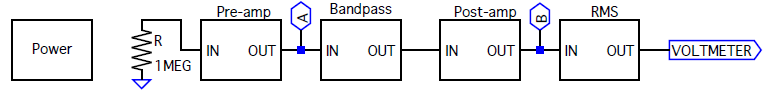
\includegraphics[width=\textwidth]{../grafici/Blocks.png}
	\vspace*{-15pt}
	\caption{Schema a blocchi del circuito complessivo.}
	\label{fig:blocks}
\end{figure}

\begin{wrapfigure}[11]{R}{0.35\textwidth}
	\vspace{-10pt}
	\centering
	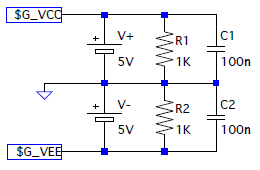
\includegraphics[width=0.35\textwidth]{../grafici/Filter.png}
	\vspace{-6pt}
	\caption{Schema di filtraggio per le alimentazioni.}
	\label{fig:powfilter}
	\vspace{-12pt}
\end{wrapfigure}

Si sono fissate le alimentazioni a $\sim \unit{5}{\volt}$ e si è montatp fra esse lo shcema di filtraggio riportato in  \cref{fig:powfilter}.

Si è proceduto con il montaggio dei singoli blocchi di circuito, che verranno illustrati individualmente nella prossima sezione.

\vspace*{-10pt}

\section{Implementazione dei blocchi di circuito}

\subsection{Pre-amplificatore}

Si è montato il circuito in \cref{fig:preamp} costituito da due amplificatori: il primo è l'integrato INA114 il cui guadagno atteso è pari a $ A_0 = (1+ 50~\kilo\Omega/R_1) = 51.6 \pm 0.5$; il secondo è costituito da un opamp con feedback sull'ingresso invertente. Il guadagno atteso di questa seconda parte di circuito è dato da $A_1 = R_3/R_2 = 14.4 \pm 0.2 $.

Le resistenze utilizzate sono riportate in \cref{tab:resistenze}.

\vspace*{-10pt}

\begin{figure}[H]
	\begin{minipage}{0.59\textwidth}
		\centering
		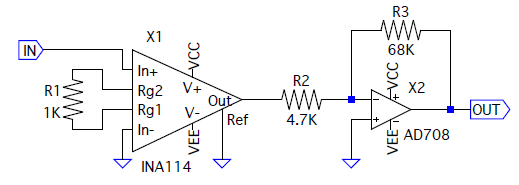
\includegraphics[width=\textwidth]{../grafici/PreAmp.png}
		\vspace{-12pt}
		\caption{Schema del circuito: pre-amplificatore.}
		\label{fig:preamp}
	\end{minipage}
	\begin{minipage}{0.39\textwidth}
		\centering
		\begin{tabular}{ccc}
			\hline
			$R_1[\Omega]$ & $R_2[k\Omega]$ & $R_3[k\Omega]$\\
			\hline
			$989\pm9$ & $4.71\pm0.05$ & $67.9\pm0.6$\\
			\hline
		\end{tabular}
		\captionof{table}{Resistenze utilizzate nel circuito in \cref{fig:preamp}.}
		\label{tab:resistenze}
	\end{minipage}
\end{figure}

\subsubsection*{Amplificazione e risposta in frequenza}
\vspace*{-5pt}
In primo luogo si è misurata la risposta in frequenza del solo amplificatore INA staccando la seconda parte del circuito e mandando al suo ingresso un'onda sinusoidale dal generatore di funzioni.
 
Come funzione modello si è scelto di prendere quella per un generico passa-basso:
\vspace*{-5pt}
\begin{equation}
\frac{A_0}{\sqrt[]{1+(\frac{f}{f_{t,0}})^2}}
\end{equation}
\vspace*{-5pt}
Le misure prese ed il fit sono riportati rispettivamente in \cref{tab:prepreamp} e in \cref{fig:prepreamp}.

\vspace*{-8pt}
\begin{figure}[H]
	\centering
	\includegraphics[width=0.6\textwidth]{../grafici/prepreamp.pdf}
	\vspace*{-10pt}
	\caption{Risposta in frequenza dell'amplificatore INA.}
	\label{fig:prepreamp}
\end{figure}
\vspace*{-10pt}

Dal fit si ottengono come risultati $A_0 = 49.805 \pm 0.004$, $f_{t,0} = 25.000 \pm 0.013~\kilo\hertz$. Il fit non è particolarmente in accordo con i dati, come risulta dal calcolo del $ \chi^2 $: osservando la \cref{fig:prepreamp} si ha che ciò è dovuto principalmente alle misure ad alta frequenza.
\footnote{Anche se meno di quello che appare in \cref{fig:prepreamp}, poiché l'asse delle ordinate è logaritmico.}
Il fit della regione a basse frequenze comunque resistuisce un valore del guadagno piuttosto preciso e in accordo con quanto atteso, mentre per la frequenza di taglio è più importante l'ordine di grandezza che la misura in sè: lo scopo è che sia nettamente esclusa dalla banda di frequenze selezionata dal filtro passabanda (vedi \cref{sec:bandpass}).

In secondo luogo si è mandata un'onda sinusoidale all'ingresso della seconda parte del circuito (prima della resistenza $R_2$) e si è studiata la sua risposta in frequenza.
Anche in questo caso come funzione modello si è scelto di prendere quella per un generico passa-basso:
\vspace*{-5pt}
\begin{equation}
\frac{A_1}{\sqrt[]{1+(\frac{f}{f_{t,1}})^2}}
\end{equation}
\vspace*{-5pt}
 Le misure prese ed il fit sono riportati rispettivamente in \cref{tab:postpreamp} e in \cref{fig:postpreamp}.
 
\vspace*{-8pt}
\begin{figure}[H]
	\centering
	\includegraphics[width=0.6\textwidth]{../grafici/postpreamp.pdf}
	\vspace*{-10pt}
	\caption{Risposta in frequenza del secondo amplificatore.}
	\label{fig:postpreamp}
\end{figure}
\vspace*{-10pt}

Dal fit si ottengono come risultati $A_1 = 14.431+/-0.003$, $f_{t,1} = 37.58+/-0.05 \kilo\hertz$.

Come nel caso precedente il fit non è ottimo, ma i parametri trovati hanno le stesse proprietà: il guadagno dipende principalmente dalla parte a bassa frequenza (in ottimo accordo con una costante, come mostrato in \cref{fig:postpreamp}), mentre la frequenza di taglio è nettamente al di fuori della regione selezionata dal filtro passabanda (mostrata in \cref{fig:FITbandpass}).

\subsection{Filtro passabanda e post-amplificatore}
\label{sec:bandpass}

\begin{wrapfigure}[18]{R}{0.55\textwidth}
	\vspace{-10pt}
	\centering
	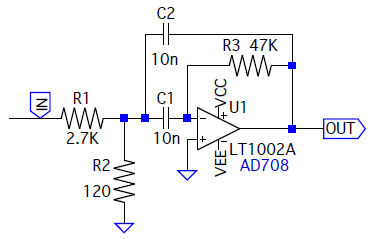
\includegraphics[width=0.55\textwidth]{../grafici/Bandpass.png}
	\vspace{-12pt}
	\caption{Schema del circuito: filtro passabanda.}
	\label{fig:bandpass}
	\vspace{-6pt}
\end{wrapfigure}

Il circuito usato per la realizzazione del filtro passabanda è stato esaminato a lezione. Non si ripetono quindi i calcoli fatti, ma si farà uso dei concetti di \textit{frequenza centrale}, \textit{larghezza di banda} e \textit{Q-valore} enunciati in tale sede.

La funzione del passabanda è quella di selezionare una banda di frequenza in modo compatibile con la definizione data nella formula di Nyquist: in assenza di un tale riferimento la banda di frequenza ci sarebbe ugualmente, dovuta alle frequenza di taglio degli op-amp e alle capacità residue dei vari elementi circuitali, ma non sarebbe ben definita.
Inoltre posizionando la frequenza centrale in modo tale che la regione selezionata non si avvicini alle frequenze di taglio dei altri elementi circuitali si riduce il problema della non idealità dei componenti, poiché nella zona d'interesse il loro comportamento approssima molto bene quello ideale.
\newline

Il circuito usato per post-amplificatore è suddiviso in due stadi, di cui il primo è costituito da un op-amp montato in configurazione di amplificatore non invertente, e il secondo è semplicemente un op-amp con feedback che ripete in uscita ciò che arriva in ingresso, in questo modo sconnette i sottocircuiti successivi da ciò che lo precede, cosicché essi non costituiscano un carico per i vari stadi di amplificazione. 

\begin{figure}[H]
	\vspace{-10pt}
	\centering
	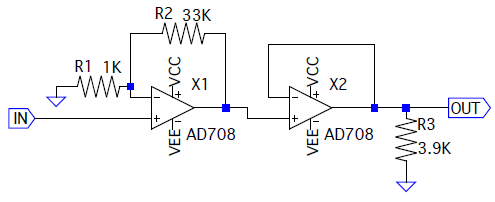
\includegraphics[width=0.7\textwidth]{../grafici/PostAmp.png}
	\vspace{-12pt}
	\caption{Schema del circuito: post-amplificatore.}
	\label{fig:postamp}
	\vspace{-6pt}
\end{figure}

\subsubsection*{Amplificazione e risposta in frequenza}

Si è misurata l'amplificazione e la risposta in frequenza dei due circuiti congiuntamente. Naturalmente il contributo maggiore alla risposta in frequenza sarà quello del passabanda, poiché gli op-amp del post-amplificatore hann un comportamento ideale fino a frequenze abbastanza elevate (molto maggiori dei $\sim 6 \kilo\hertz $ della frequenza centrale).

Si riportano in \cref{fig:FITbandpass} i dati presi per la risposta in frequenza e il fit che si è fatto di essi (il grafico su cui sono mostrati è bilogaritmico).
La funzione di cui stato eseguito il fit è:
\[ A(f) = A_2^\star \frac{f}{\sqrt{(f^2-f_0^2)^2 + \left(\frac{f_0 f}{Q}\right)^2}} \]

e i parametri trovati dal fit sono:
\[ A_2^\star=(1.495 \pm 0.012)\cdot10^5 \qquad Q=57.6 \pm 1.9 \qquad f_0=6.084 \pm 0.007~\kilo\hertz  \]
da cui si può dedurre il valore dell'amplificazione di centro banda $ A_{2,0} $ e la larghezza di banda $ \Delta f $:
\[ A_{2,0} = 186.5 \pm 2.2	\qquad	\Delta f \]
\vspace*{-30pt}
\begin{figure}[H]
	\centering
	\includegraphics[width=0.7\textwidth]{../grafici/passabanda.pdf}
	\vspace*{-5pt}
	\caption{Amplificazione e risposta in frequenza degli stadi passabanda e post-amplificatore in serie.}
	\label{fig:FITbandpass}
\end{figure}

\subsection{Convertitore RMS}
\vspace*{-30pt}
\begin{figure}[H]
	\begin{minipage}{0.34\textwidth}
		\vspace{-10pt}
		\centering
		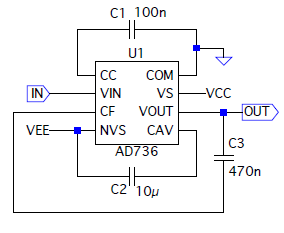
\includegraphics[width=\textwidth]{../grafici/RMSconverter.png}
		\vspace{-12pt}
		\caption{Schema del circuito: convertitore RMS.}
		\label{fig:RMSconv}
		\vspace{-6pt}
	\end{minipage}
	\begin{minipage}{0.64\textwidth}
		\centering
		\includegraphics[width=\textwidth]{../grafici/calibrazione.pdf}
		\vspace*{-20pt}
		\caption{Fit della calibrazione del convertitore RMS.}
		\label{fig:FitRMS}
	\end{minipage}
\end{figure}

Il convertitore RMS è stato realizzato tramite un apposito integrato (AD736), montato nella configurazione mostrata in \cref{fig:RMSconv}.
\vspace*{-8pt}
\subsubsection*{Calibrazione}

Si è eseguita la calibrazione della lettura data in uscita dal circuito in \cref{fig:RMSconv}, confrontando la lettura del multimetro di questa tensione con il valore RMS calcolato dall'apposita funzione dell'oscilloscopio.
Il risultato del fit è riportato in \cref{fig:FitRMS}, mentre i valori ottenuti sono:
\[ m = 0.870 \pm 0.005	\qquad	q = -(1.38+/-0.10) \milli\volt	\qquad	\chi^2/DOF = 15.72 / 16 \]
dove $ m $ è il coefficiente angolare della retta e $ q $ la sua intercetta.


\section{Misura della costante di Boltzmann}
\vspace*{-5pt}
Si sono montati i vari circuiti tutti insieme, come schematizzato dalla \cref{fig:blocks}. Si è misurato il valore $V_{RMS}$ in uscita al circuito al variare della resistenza in ingresso. Per ogni resistenza sono stati presi più valori di $V_{RMS}$ poiché la misura oscillava molto. Si è poi effettuata una media dei valori presi. I dati ottenuti sono riportati in \cref{tab:lastfitav}.
\vspace*{-10pt}
\begin{table}[H]
	\centering
	\begin{tabular}{cccc}
		\hline
		R[k$\Omega$] & $\delta$R [k$\Omega$] & $V_{RMS}[mV]$  & $\delta$$V_{RMS}[mV]$ \\
		\hline
		0.985 & 0.009 & 35 & 1 \\
		1.18 & 0.01 & 36.1 & 0.5 \\
		1.48 & 0.01 & 36.7 & 0.8 \\
		2.14 & 0.03 & 37.5 & 0.6 \\
		3.26 & 0.04 & 38.9 & 0.7 \\
		3.83 & 0.04 & 41.3 & 0.9 \\
		4.68 & 0.05 & 43.9 & 0.9 \\
		5.59 & 0.05 & 46.7 & 0.8 \\
		6.71 & 0.06 & 50.3 & 0.8 \\
		8.11 & 0.07 & 51.1 & 0.8 \\
		9.91 & 0.09 & 54 & 1 \\
		9.97 & 0.08 & 58 & 2 \\
		11.8 & 0.1 & 62 & 2 \\
		17.9 & 0.2 & 72 & 2 \\
		\hline
	\end{tabular}
	\caption{Valori delle resistenze utilizzate e del potenziale all'uscita del circuito.}
	\label{tab:lastfitav}
\end{table}
\vspace*{-5pt}
Le relazioni attese che legano $V_{RMS}$, le resistenze utilizzate, i guadagni ottenuti e la costante di Boltzmann $k_b$ sono le seguenti:
\vspace*{-8pt}
\begin{equation}
V_{RMS} = V_{0n} \sqrt[]{1+\frac{R}{R_T}+\frac{R^2}{R_n ^2}}
\label{fitt}
\end{equation}
dove R è la resistenza in ingresso, $R_T, V_0n e R_n$ sono parametri che si otterranno dal fit a questa funzione.
\begin{equation}
V_0n = A V_n
\label{resnull}
\end{equation}
che rappresenta il rumore in uscita a resistenza nulla. Il Guadagno $A$ è quello complessivo di tutto il circuito, cioè $A = A_0 A_1 A_2 A_3 = (1.17\pm0.02)e+05 $.
\vspace*{-10pt}
\begin{equation}
R_T = \frac{V_n^2}{4k_b T \Delta f} = \frac{V_0n^2}{4k_b A_0 T \Delta f}
\label{kb}
\end{equation}
che è la resistenza equivalente del rumore serie dell'amplificatore riferito all'ingresso.

Si è quindi effettuato un fit alla $\eqref{fitt}$ ottenendo come risultati $V_0n = 0.0329\pm0.0007 V$ , $R_T = (7\pm1)e+03 \Omega $, $R_n = (1.5\pm 0.2)e+04 \Omega$, $\chi ^2 /DOF$ = 93/11. Il $\chi ^2$ risulta essere leggermente alto; si ritiene che ciò sia dovuto ad una sottostima degli errori.
%... lascio così come commento? chi2 senza media = 17.

Il grafico è mostrato in \cref{fig:lastfit}.
\vspace*{-10pt}
\begin{figure}[H]
	\centering
	\includegraphics[width=0.7\textwidth]{../grafici/lastfit.pdf}
	\vspace*{-15pt}
	\caption{Fit di $V_{RMS}$ in funzione di R.}
	\label{fig:lastfit}
\end{figure}



\subsection{Stima diretta dell'amplificazione \\e risposta in frequenza del circuito complessivo}
Si è misurata direttamente l'amplificazione e la risposta in frequenza del circuito complessivo mandando segnali molti piccoli in ingresso utilizzando un partitore 1000:1 (si sono utilizzate a tal proposito le resistenze $R_1 = 9.91\pm0.09 k\Omega $ e $R_2 = 10.1\pm0.4 \Omega$).
I dati raccolti sono mostrati in \cref{tab:totamp}.

Si è effettuato un fit su questi dati per trovare l'amplificazione complessiva del circuito. Si è modellizzato tutto il circuito come se fosse un unico passabanda amplificato, con amplificatori ideali (con frequenza di taglio costante). La funzione di fit è la seguente:
\begin{equation}
\frac{1}{\sqrt{1+(\frac{f}{f_t})^2}} \frac{A^\star f}{\sqrt{(f - f_0)^2+ \frac{f^2 f_0^2}{Q} )}}
\end{equation}

Questa stima potrebbe ulteriormente essere migliorata utilizzando come modello il prodotto tra le varie funzioni di trasferimento degli amplificatori (tutti con frequenze di taglio diverse) e il passabanda, ma come si può notare dal fit e dai suoi risultati, anche il modello utilizzato è fitta bene i dati. Il grafico è mostrato in \cref{fig:ampltot} e i risultati in \cref{tab:risult}.

\begin{figure}[H]
	\centering
	\includegraphics[width=0.7\textwidth]{../grafici/amp_alternativa_imp.pdf}
	\caption{fit dell'amplificazione totale in funzione della frequenza del segnale in ingresso al circuito.}
	\label{fig:ampltot}
\end{figure}

\begin{table}[H]
	\centering
	\begin{tabular}{c|c|c|c|c}
	$A^\star$ & Q & $f_0[Hz]$ & $f_t[Hz]$ & $\chi^2/DOF$ \\
	\hline
	(1.57$\pm$0.06)e+08 & 9.0$\pm$0.4 & 6794$\pm$35 & (9.1$\pm$0.8)e+03 & 16/19 \\
	\end{tabular}
	\caption{Risultati del fit per valutare l'amplificazione complessiva del circuito e la sua risposta in frequenza.}
	\label{tab:risult}
\end{table}

I valori ottenuti per l'amplificazione totale e per la banda passante sono rispettivamente A = (4.84$\pm$0.08)e+04 e $\Delta f$ = (4.75$\pm$0.23)e+03 Hz.

%non sono sicuro dei risultati che ho messo soprattutto delta f che esce 3 ordini di grandezza diversa, per piacere controllate ed aggiustate.


\subsection{Risultati finali}
A questo punto, utilizzando la \eqref{resnull} e la \eqref{kb} si è ricavata la costante di Boltzmann con entrambi i metodi sopra descritti. Si sono ottenuti come risultati rispettivamente $k_b = (1.44\pm0.19)e-23 J/K$ e $k_{b,1000:1} = (1.17\pm0.16)e-23~J/K $. Il valore atteso per la costante di Boltzmann è $k_b$ = 1.380e-23 J/K. I risultati ottenuti sono entrambi compatibili con il valore atteso. 

\pagebreak

\section{Appendice: Dati Acquisiti}
Si riportano qui le tabelle dei dati usati per i fit e i grafici.

\begin{table}[H]
	\centering
	\input{../tabelle/tab_prepreamp.txt}
	\caption{.}
	\label{tab:prepreamp}
\end{table}

\begin{table}[H]
	\centering
	\input{../tabelle/tab_postpreamp.txt}
	\caption{.}
	\label{tab:postpreamp}
\end{table}

\begin{figure}
	\begin{minipage}{0.64\textwidth}
		\begin{table}[H]
			\centering
			\input{../tabelle/tab_passabanda.txt}
			\caption{.}
			\label{tab:bandpass}
		\end{table}
	\end{minipage}
	\begin{minipage}{0.34\textwidth}
		\begin{table}[H]
			\centering
			\input{../tabelle/tab_calibrazioneRMS.txt}
			\caption{.}
			\label{tab:RMScal}
		\end{table}
	\end{minipage}
\end{figure}

\begin{table}[H]
	\centering
	\input{../tabelle/tab_totamp.txt}
	\caption{Valori delle frequenze utilizzate e del potenziale in uscita al circuito utilizzando un partitore 1000:1.}
	\label{tab:totamp}
\end{table}

\pagebreak

L'errore sulle tensioni nelle prossime due tabelle è stato ottenuto considerando l'errore di calibrazione dello strumento, che naturalmente non è stato considerato come errore statistico\footnote{Perché non lo è.} nei fit eseguiti.
L'errore non di calibrazione corrisponde per tutte le tensioni trovate all'ultimo digit sulla lettura.

\begin{table}[H]
	\centering
	\input{../tabelle/tab_lastfit.txt}
	\caption{.}
	\label{tab:lastfit}
\end{table}

\begin{table}[H]
	\centering
	\input{../tabelle/tab_lastfit1.txt}
	\caption{.}
	\label{tab:lastfit1}
\end{table}

\end{document}